\section{Introduction}

This document specifies the design for a Snake game programmed in C++ using the SFML library. It is also used for practicing the creation of a Game Design Document (GDD). It contains game design information including lose conditions, game states, controls, and a development task list.

\subsection{References}
\begin{enumerate}
	\item \url{https://www.gamedevs.org/uploads/grand-theft-auto.pdf}
	\item \url{https://www.nuclino.com/articles/game-design-document-template}
\end{enumerate}

\section{Specification}

\subsection{Concept}
Snake is an addictive game where the goal is to achieve as many points as possible.

\subsection{Story}
The classic Snake game has no real story. The setting is a space environment: the snake must constantly move and eat to survive.

\subsection{Game Structure}
There is one gameplay screen, in addition to title and menu screens. The background is a static space image. The snake can move beyond one edge of the screen and reappear at the opposite edge. Static obstacles can kill the snake when touched.

\subsection{Player}
The game is designed for one player at a time. Multiple players can compete for the high score.

\subsection{Action}
The player steers the snake while it moves continuously. The snake becomes faster as the game progresses. Pellets have a limited lifetime, so the player must prioritize which pellets to collect. A point multiplier may be awarded when multiple pellets are collected within a short period.

The player must avoid the snake's own body and obstacles. The game becomes more difficult as the snake grows and its speed increases.

\subsection{Objective}
The objective is to stay alive and achieve the highest possible score by eating pellets.

\subsection{Graphics}
The graphics are two-dimensional. The game window is no larger than 1280 by 1024 pixels. Text uses the ``Retro Stereo Wide'' font.

Pellets change color before disappearing if they are not collected. The snake becomes white when dying. A panel along the upper edge of the screen displays the score so that it is easy to read.

\section{Gameplay}

\subsection{World}
The world is static and consists of a single screen. The snake can wrap around the screen: when it travels beyond one edge, it returns from the opposite edge.

The music is calm. The original design document identifies ``Life Stream'' from \emph{Final Fantasy VII} by Nobuo Uematsu as the intended music.

\subsection{Objects}

\subsubsection{Pellets}
Pellets are objects in the world that the snake can eat to grow. They provide points, and the player should collect as many as possible as quickly as possible.

\subsubsection{Snake Head}
The snake's head is controlled by the player, while the body follows it. The head is always moving and accelerates over time; the player controls its rotation.

\begin{figure}[htbp]
	\centering
	
\includegraphics[width=6.61mm,height=6.61mm]{latex/images/image1.png}
	\caption{Snake head example.}
\end{figure}

\subsubsection{Snake Body}
Body parts are added behind the head and follow it like a tail. The snake starts with two body parts.

\begin{figure}[htbp]
	\centering
	
\includegraphics[width=6.61mm,height=6.61mm]{latex/images/image2.png}
	\caption{Snake body example.}
\end{figure}

\subsection{Controls}
The player uses the arrow keys to steer the snake. The mouse is used to navigate the menus. Pressing \texttt{Esc} during gameplay pauses the game and displays the in-game menu.

\subsection{Menus}

\subsubsection{Main Menu}
\begin{description}
	\item[Start] Starts the game.
	\item[High Score] Shows the high-score list.
	\item[Quit] Closes the game.
\end{description}

\begin{figure}[htbp]
	\centering
	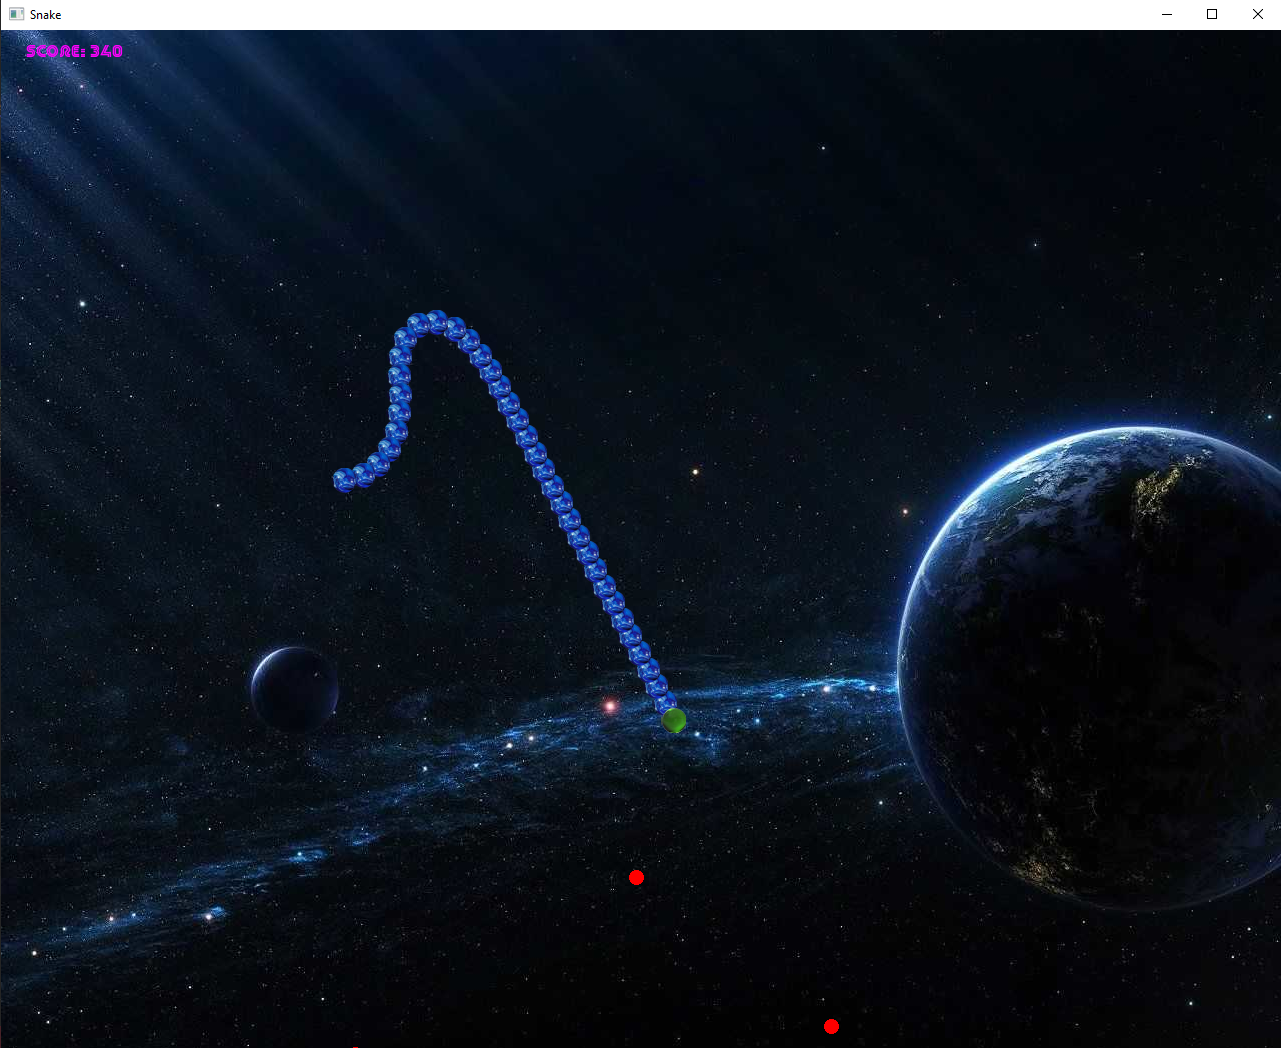
\includegraphics[width=0.9\textwidth,height=0.45\textheight,keepaspectratio]{latex/images/image3.png}
	\caption{Early build of the game.}
\end{figure}

\subsubsection{Pause Menu}
\begin{description}
	\item[Resume] Resumes the game.
	\item[Restart] Restarts the game, resets the score to zero, restores the starting speed, and makes the snake small again.
	\item[Quit] Closes the game.
\end{description}

\section{Development}

\subsection{Tools}
The code is written in C++ using the SFML API as the graphics and game engine. The game is developed in Microsoft Visual Studio. GIMP is used to create sprites.

The project intentionally uses an older C++ memory-allocation style for training. Smart pointers are not used in the original design.

\subsection{Algorithms}

\subsubsection{Body Following the Head}
Each body part follows the previous part using the following calculation:

\begin{figure}[htbp]
	\centering
	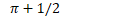
\includegraphics[width=0.8\textwidth,height=0.25\textheight,keepaspectratio]{latex/images/image4.png}
	\caption{Body-following diagram.}
\end{figure}

\begin{verbatim}
dx = Head->getXpos() - body->getXpos();
dy = Head->getYpos() - body->getYpos();
angle = atan2f(dy, dx);

Body->setXpos(Head->getXpos() - cosf(angle) * Body->getRadius() * 1.5f);
Body->setYpos(Head->getYpos() - sinf(angle) * Body->getRadius() * 1.5f);
\end{verbatim}

The next body part uses the same calculation, but uses the position of the previous body part instead of the head.

\subsubsection{Head Rotation}
The head is steered using the following calculation:

\begin{figure}[htbp]
	\centering
	
\includegraphics[width=0.8\textwidth,height=0.25\textheight,keepaspectratio]{latex/images/image5.png}
	\caption{Head rotation diagram.}
\end{figure}

\begin{verbatim}
angle = angle + RotationSpeed;

xVel = cos(Angle);
yVel = sin(Angle);

xPos = xPos + xVel;
yPos = yPos + xVel;
\end{verbatim}

The sign of \texttt{RotationSpeed} depends on player input. Right input applies positive rotation and left input applies negative rotation.

\subsubsection{Circular Collisions}
Circular collision detection is used for objects such as the snake and pellets.

\begin{figure}[htbp]
	\centering
	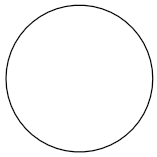
\includegraphics[width=0.8\textwidth,height=0.25\textheight,keepaspectratio]{latex/images/image6.png}
	\caption{Circular collision diagram.}
\end{figure}

\subsubsection{Circle Against Box Collisions}
Circle-against-box collision detection is intended for collisions between circular game objects and rectangular obstacles.

\begin{figure}[htbp]
	\centering
	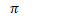
\includegraphics[width=0.8\textwidth,height=0.25\textheight,keepaspectratio]{latex/images/image7.png}
	\caption{Circle-against-box collision diagram.}
\end{figure}

\begin{figure}[htbp]
	\centering
	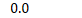
\includegraphics[width=0.8\textwidth,height=0.25\textheight,keepaspectratio]{latex/images/image8.png}
	\caption{Additional collision reference diagram.}
\end{figure}

\begin{figure}[htbp]
	\centering
	
\includegraphics[width=0.8\textwidth,height=0.25\textheight,keepaspectratio]{latex/images/image9.png}
	\caption{Additional collision reference diagram.}
\end{figure}

\begin{figure}[htbp]
	\centering
	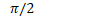
\includegraphics[width=0.8\textwidth,height=0.25\textheight,keepaspectratio]{latex/images/image10.png}
	\caption{Additional collision reference diagram.}
\end{figure}

\section{Development Task List}
\begin{itemize}
	\item Add obstacles.
	\item Add music.
	\item Add sound effects.
	\item Implement a dynamically growing snake.
	\item Add a pause menu.
	\item Add a main menu.
\end{itemize}
